\documentclass[article]{jss}
\usepackage[utf8]{inputenc}

\providecommand{\tightlist}{%
  \setlength{\itemsep}{0pt}\setlength{\parskip}{0pt}}

\author{
Anna Michalek\\European Central Bank \And Alain Quartier-la-Tente\\Insee
}
\title{\pkg{RJDemetra}: An \proglang{R} Interface To \proglang{JDemetra+}
Seasonal Adjustment Software}

\Plainauthor{Anna Michalek, Alain Quartier-la-Tente}
\Plaintitle{RJDemetra: An R Interface To JDemetra+ Seasonal Adjustment Software}

\Abstract{
\pkg{RJDemetra} provides an interface between \proglang{R} and
\proglang{JDemetra+}, the only seasonal and trading days adjustment
software officially recommended by Eurostat to the members of the
European Statistical System and the European System of Central Banks.
\pkg{RJDemetra} offers access to main options and outputs of
\proglang{JDemetra+}, including the two leading seasonal adjustment
methods TRAMO-SEATS and X-13ARIMA. Thus, it is possible to use
user-defined or pre-specified specification and to estimate a RegARIMA
model including automatic outlier and ARIMA detection, moving holiday
effects and user-defined regressors. With \pkg{RJDemetra} it is also
possible to read and write \proglang{JDemetra+} workspaces that are used
in production. Thus, thanks to all the resources available in
\proglang{R}, it offers large possibilities to develop tools to improve
the production of seasonal adjusted series.
}

\Keywords{\proglang{R}, seasonal adjustment, calendar effects, ARIMA, outliers, time series}
\Plainkeywords{R, seasonal adjustment, calendar effects, ARIMA, outliers, time series}

%% publication information
%% \Volume{50}
%% \Issue{9}
%% \Month{June}
%% \Year{2012}
%% \Submitdate{}
%% \Acceptdate{2012-06-04}

\Address{
    }

% Pandoc header

\usepackage{amsmath} \usepackage{booktabs} \usepackage{longtable} \usepackage{array} \usepackage{multirow} \usepackage{wrapfig} \usepackage{float} \usepackage{pdflscape} \usepackage{tabu} \usepackage{threeparttable} \usepackage{threeparttablex} \usepackage[normalem]{ulem} \usepackage{makecell}

\begin{document}

\hypertarget{introduction}{%
\section{Introduction}\label{introduction}}

Since the 20th century, more and more infra-annual statistics are
produced, especially by national institutes, to analyse the short-term
evolution of economies. It is for example the case of the gross domestic
product (GDP), unemployment rate, household consumption of goods and
industrial production indices. However, most of those time series are
affected by seasonal and trading days effects. A seasonal effect is an
effect that occurs in the same calendar month with similar magnitude and
direction from year to year. For instance, automobile production is
usually lower during summer, due to holidays, and chocolate sales are
usually higher in December, due to Christmas. Trading days effect
appears when a time series is affected by calendar month's weekday
composition. For example retail sales are usually higher on Saturday,
thus they are likely to be higher in months with a surplus of weekend
days.

Seasonal and trading days effects can hamper the analysis of
infra-annual movements of a time series or the spatial comparison. This
is the reason why time series are often seasonally and trading days
adjusted, where seasonal adjustment is the process of removing the
effects of seasonal and trading day fluctuations.

\hypertarget{theory-behind-seasonal-adjustment}{%
\section{Theory behind seasonal
adjustment}\label{theory-behind-seasonal-adjustment}}

The most popular seasonal adjustment methods are TRAMO-SEATS\footnote{The
  program \proglang{TRAMO-SEATS} was developed by Gianluca Caporello and
  Agustin Maravall --- with programming support from Domingo Perez and
  Roberto Lopez --- at the Bank of Spain. It is based on the program
  TRAMO-SEATS, previously developed by Victor Gomez and Agustin
  Maravall.} \citep{gomez1996programs, caporello2004program}, a
parametric method based on ARIMA models, and X-13ARIMA\footnote{The
  program \proglang{X-13ARIMA} is a produced, distributed, and
  maintained by the US-Census Bureau.}
\citep{findleyx12, ladiray1999x11en}, a non-parametric method based on
moving averages. Both methods are recommended by Eurostat and the
European Central Bank (ECB) for adjusting economic indicators. These two
methods proceed in two steps, summarized in figure
\ref{fig:2_step_proc}.

\begin{figure}[htb]
\centering
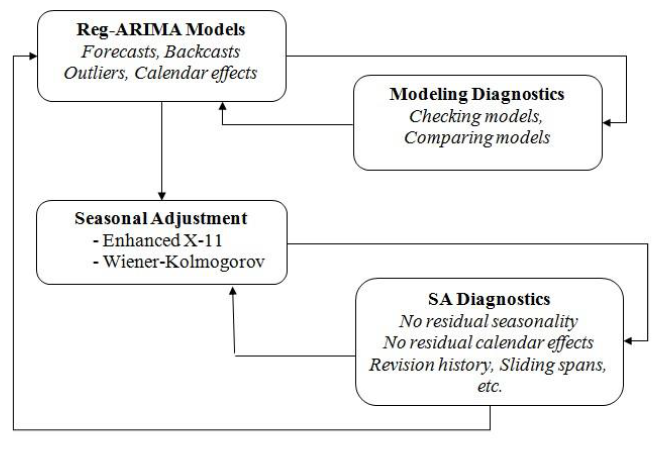
\includegraphics[scale=0.8]{img/sa_2_steps.PNG} 
\caption{X-13ARIMA and TRAMO-SEATS 2-step process: pre-adjustment and decomposition.}
\label{fig:2_step_proc}
\end{figure}

The \textbf{first step}, called \textbf{pre-adjustment} or
\textbf{linearisation}, consists of pre-adjusting the time series by
removing the deterministic effects and estimating missing observations.
Next, in the \textbf{second part} of seasonal adjustment, called the
\textbf{decomposition}, the pre-adjusted series is decomposed in order
to determine the seasonal component. As a result of this process, the
final seasonally adjusted series shall be free of seasonal and
calendar-related movements.

The pre-adjustment step is very similar in X-13ARIMA and in TRAMO-SEATS
(section \ref{pre-adjustment}), whereas the decomposition differs
between the two methods. In X-13ARIMA, the X-11 algorithm decomposes the
time series by means of linear filters (section \ref{sa-x11}). In
TRAMO-SEATS, SEATS (Signal Extraction in ARIMA Time Series) decomposes
the observed series with a ARIMA-model based method (section
\ref{sa-seats}).

\hypertarget{pre-adjustment}{%
\subsection{Pre-adjustment with TRAMO and RegARIMA
models}\label{pre-adjustment}}

As aforementioned, the \textbf{first step} of seasonal adjustment
consists of pre-adjusting the time series by removing from it the
deterministic effects like outliers, calendar and regression effects.
This step estimates also the missing observations, as well as produces
forecasts and backasts of the pre-adjusted series which allows applying
linear filters at both ends of the series in the decomposition part of
the seasonal adjustment. All this is achieved with a \textbf{RegARIMA}
model (model with ARIMA errors) as specified below.

\[z_t=y_t\beta+x_t\] where

\begin{itemize}
\tightlist
\item
  \(z_t\) - is the original series;
\item
  \(\beta = (\beta_1,\dots,\beta_n)\) - a vector of regression
  coefficients;
\item
  \(y_t = (y_{1t},\dots,y_{nt})\) - \(n\) regression variables
  (outliers, calendar effects, user-defined variables);
\item
  \(x_t\) - a disturbance that follows the general ARIMA process:
\item
  \(\phi(B)\delta(B)x_t=\theta(B)a_t\); \(\phi(B), \delta(B)\) and
  \(\theta(B)\) are the finite polynomials in \(B\); \(a_t\) is a
  white-noise variable with zero mean and a constant variance.
\end{itemize}

The polynomial \(\phi(B)\) is a stationary autoregressive (AR)
polynomial in \(B\), which is a product of the stationary regular AR
polynomial in \(B\) and the stationary seasonal polynomial in \(B^s\):

\[\phi(B)=\phi_p(B)\Phi_{bp}(B^s)=(1+\phi_1B+\dots+\phi_pB^p)(1+\Phi_1B^s+\dots+\Phi_{bp}B^{bps})\]

where:

\begin{itemize}
\tightlist
\item
  \(p\) - number of regular AR terms (in the package and in
  \proglang{JDemetra+} \(p \le 3\));
\item
  \(bp\) - number of seasonal AR terms (in the package and in
  \proglang{JDemetra+} \(bp \le 1\));
\item
  \(s\) - number of observations per year (frequency of the time
  series).
\end{itemize}

The polynomial \(\theta(B)\) is an invertible moving average (MA)
polynomial in \(B\), which is a product of the invertible regular MA
polynomial in \(B\) and the invertible seasonal MA polynomial in
\(B^s\):

\[\theta(B)=\theta_q(B)\Theta_{bq}(B^s)=(1+\theta_1B+\dots+\theta_qB^q)(1+\Theta_1B^s+\dots+\Theta_{bq}B^{bqs})\]

where:

\begin{itemize}
\tightlist
\item
  \(q\) - number of regular MA terms (in the package and in
  \proglang{JDemetra+} \(q \le 3\));
\item
  \(bq\) - number of seasonal MA terms (in the package and in
  \proglang{JDemetra+} \(bq \le 1\));
\end{itemize}

The polynomial \(\delta(B)\) is the non-stationary AR polynomial in
\(B\) (unit roots):

\[\delta(B)=(1-B)^d(1-B^s)^{d_s}\]

where:

\begin{itemize}
\tightlist
\item
  \(d\) - regular differencing order (in the package and in
  \proglang{JDemetra+} \(d \le 1\));
\item
  \(d_s\) - seasonal differencing order (in the package and in
  \proglang{JDemetra+} \(d_s \le 1\));
\end{itemize}

Furthermore, in this step an automatic modelling is implemented (in both
methods) to: determine the decomposition of the series, detect outliers
and calendar effects and to adjust residuals to an ARIMA models. A
detailed description can be found in \cite{gomez1998automatic}.

\hypertarget{sa-x11}{%
\subsection{Decomposition with X-11}\label{sa-x11}}

In this step, the pre-adjusted series (\(y\)) is decomposed into the
following components: trend-cycle (\(t\)), seasonal component (\(s\))
and irregular component (\(i\)), where the decomposition can be:

\begin{itemize}
\tightlist
\item
  additive (\(y = t + s + i\));\\
\item
  multiplicative (\(y = t \times s \times i\));\\
\item
  log-additive (\(\log(y) = \log(t) + \log(s) + \log(i)\));\\
\item
  pseudo-additive (\(y = t \times (s + i - 1)\)).
\end{itemize}

In X-11, which is an iterative non-parametric method, the decomposition
is achieved by means of linear filters
\citep{findleyx12, ladiray1999x11en}. The basic procedure consists of a
simple 3-step algorithm:

\begin{enumerate}
\def\labelenumi{\arabic{enumi})}
\tightlist
\item
  Estimate the trend by means of moving averages;
\item
  Remove the trend and leave the seasonal and irregular components;
\item
  Estimate the seasonal component using moving averages.
\end{enumerate}

At each step, the program selects a moving average among a large set of
predefined smoothers, according to the characteristics of the series.
X-11 also incorporates an automatic detection and correction of
(additive) outliers to make the use of linear filters more robust.

\hypertarget{sa-seats}{%
\subsection{Decomposition with SEATS}\label{sa-seats}}

SEATS is a program for decomposing time series into their unobserved
components following an ARIMA model that extracts from a time series its
different signals \citep{gomez1996programs, caporello2004program}. The
decomposition can be:

\begin{itemize}
\tightlist
\item
  additive or ;
\item
  multiplicative (equivalent to an additive model after taking the
  logarithm).
\end{itemize}

SEATS decomposes the linearized series into the following components:

\begin{itemize}
\tightlist
\item
  \textbf{trend-cycle component:} captures the low-frequency variation
  of the series and displays a spectral peak at frequency 0;\\
\item
  \textbf{seasonal component:} captures the spectral peaks at seasonal
  frequencies;\\
\item
  \textbf{irregular component:} captures erratic, white-noise behaviour,
  and hence has a flat spectrum;\\
\item
  \textbf{transitory component:} a zero-mean stationary component that
  picks up transitory fluctuations that should not contaminate the
  trend-cycle or seasonal component and are not white-noise.
\end{itemize}

The components are determined and fully derived from the structure of
the ARIMA model for the observed series.

The decomposition assumes orthogonal components, and each one will have
in turn an ARIMA expression. In order to identify the components, it is
required that (except for the irregular one) they are clean of noise.
This is called the ``canonical'' property, and implies that no additive
white noise can be extracted from a component that is not the irregular
one. The variance of the latter is, in this way, maximized, and, on the
contrary, the trend-cycle and seasonal component are as stable as
possible (compatible with the stochastic nature of model).

\section[JDemetra+ and RJDemetra]{\proglang{JDemetra+} and \pkg{RJDemetra}}

\proglang{JDemetra+} is a tool for seasonal adjustment (SA) developed by
the National Bank of Belgium (NBB) in cooperation with the Deutsche
Bundesbank and Eurostat in accordance with the Guidelines of the
European Statistical System (ESS) \citep{eurostat2015guidelines}. It
implements the concepts and algorithms used in the two leading seasonal
adjustment methods: TRAMO-SEATS and X-13ARIMA. Those methods have been
re-engineered using an object-oriented approach that facilitates
estimations handling, extensions and modifications.

\proglang{JDemetra+} has been
\href{https://ec.europa.eu/eurostat/cros/system/files/Jdemetra_\%20release.pdf}{officially
recommended}, since 2 February 2015, to the members of the ESS and the
European System of Central Banks as software for seasonal and calendar
adjustment of official statistics.

Besides seasonal adjustment, \proglang{JDemetra+} bundles other time
series models that are useful in the production and analysis of economic
statistics, including for instance outlier detection, nowcasting,
temporal disaggregation or benchmarking. More details on the methodology
used in \proglang{JDemetra+} can be found in the \proglang{JDemetra+}
manuals and user guides
\citep{grudkowska2015jdemetrarm, grudkowska2015jdemetraug}.

The package \pkg{RJDemetra} \citep{RJDemetra} provides an R interface to
the seasonal adjustment software \proglang{JDemetra+}. \pkg{RJDemetra}
uses Java libraries of \proglang{JDemetra+}, therfore relies on the
\pkg{rJava} \citep{rJava} package. Consequently Java SE 8 or later
versions are required. The package allows to:

\begin{itemize}
\tightlist
\item
  perform seasonal adjustment with TRAMO-SEATS and X-13ARIMA with
  pre-defined (section \ref{pre-def-est}) and user-defined
  specifications (section \ref{user-def-spec});\\
\item
  access all outputs available in \proglang{JDemetra+} (section
  \ref{sa-obj-struc});\\
\item
  import and export \proglang{JDemetra+} workspaces (section
  \ref{manipulate-workspace}).
\end{itemize}

It can be installed from CRAN:

\begin{CodeChunk}

\begin{CodeInput}
R> install.packages("RJDemetra")
\end{CodeInput}
\end{CodeChunk}

The development version can be installed from GitHub with \pkg{devtools}
\citep{devtools}:

\begin{CodeChunk}

\begin{CodeInput}
R> devtools::install_github("jdemetra/rjdemetra")
\end{CodeInput}
\end{CodeChunk}

For the moment the seasonal and trading day adjustment can only be done
for monthly, bimonthly (for TRAMO-SEATS only), quarterly and half-yearly
data. By the end of 2020 \proglang{JDemetra+}, and therefore
\pkg{RJDemetra}, will be extended to be compatible with every biannual
frequency (daily, weekly, etc.).

\hypertarget{dataset}{%
\subsection{Dataset}\label{dataset}}

The package \pkg{RJDemetra} includes the \texttt{sts\_inpr\_m} database
of the Eurostat, which contains monthly industrial production indices in
manufacturing for the European Union. It contains 37 time series from
January 1990 to December 2017 which are considered to be affected by
seasonal and trading days effects. The data are \code{ts} objects and
can be accessed using the \code{ipi_c_eu} object. The following snippet
of code plots the industrial production index of the euro area (EA19):

\begin{CodeChunk}

\begin{CodeInput}
R> library(RJDemetra)
R> plot(ipi_c_eu[, "EA19"])
\end{CodeInput}


\begin{center}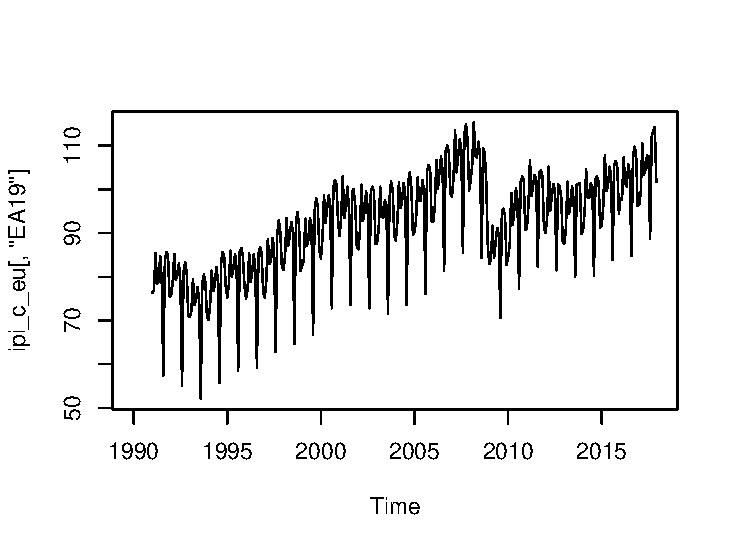
\includegraphics{img/img-basic_raw_data_plot-1} \end{center}

\end{CodeChunk}

\hypertarget{print-styling}{%
\subsection{Print styling}\label{print-styling}}

By default, a colour styling is used for the \code{print} methods of the
objects created by \pkg{RJDemetra}. It can causes troubles with some
outputs --- for example with \pkg{rmarkdown} \citep{rmarkdown} --- and
can be disabled in each \code{print} function with the argument
\code{enable_print_style = FALSE} or setting the global option
\code{enable_print_style} to \code{FALSE}:

\begin{CodeChunk}

\begin{CodeInput}
R> options(enable_print_style = FALSE)
\end{CodeInput}
\end{CodeChunk}

\hypertarget{pre-def-est}{%
\section{Estimate a pre-defined RegARIMA and seasonal adjustment
model}\label{pre-def-est}}

As in \proglang{JDemetra+}, \pkg{RJDemetra} allows to perform seasonal
adjustment using pre-defined model specifications that are the most
commonly used specifications and are recommended to users for the start
of their analysis. They are separately defined for TRAMO-SEATS and
X-13ARIMA methods. It is also possible to perform only the first step of
seasonal adjustment; i.e.~the RegARIMA estimation. The pre-defined model
specifications are described in detail in tables \ref{tab:pre_def_ts}
and \ref{tab:pre_def_x13}. They are identical for pre-adjustment (column
1) and for seasonal adjustment (column 2). The settings described in
tables \ref{tab:pre_def_ts} and \ref{tab:pre_def_x13} refer to:

\begin{itemize}
\tightlist
\item
  Transformation: test to choose between an additive decomposition (no
  transformation) and a multiplicative decomposition (logarithmic
  transformation).\\
\item
  Pre-adjustment for leap-year (not available for TRAMO): in the case of
  a multiplicative decomposition a correction of the February values is
  applied to the original series (before transformation). The original
  values in February are multiplied by \(\frac{28.25}{29}\) for leap
  years, by \(\frac{28.25}{28}\) for non-leap years and values for other
  months are not modified. In the case of multiplicative models, this is
  equivalent to adding a leap year regressor
  \citep{bell1992lengthmonthadj}.\\
\item
  Working days/trading days: test for the presence of working
  day/trading day effects. In TRAMO an automatic choice between working
  days and trading days regressors is done with ``RSAFull''.\\
\item
  Easter: pre-test for the presence of the Easter effect. For
  TRAMO-SEATS the default length of the Easter effect is 6 days and for
  X-13ARIMA an automatic detection of the duration is done (1, 8 or 15
  days).\\
\item
  Outliers: an automatic identification of three types of outliers: AO
  (additive outlier), LS (level shift) and TC (transitory change), using
  a default critical value. The automatic identification of SO (seasonal
  outlier) is not enabled by default.\\
\item
  ARIMA model: the choice between fixing the ARIMA model structure to
  (0,1,1)(0,1,1) (Airline model) or searching for ARIMA model orders
  using an automatic model identification procedure. The Airline model
  is used as a default model in several TRAMO-SEATS and X-13ARIMA
  specifications as it has been shown in several studies that it is
  appropriate in many cases for real seasonal monthly or a quarterly
  time series. Moreover, the Airline model approximates well many other
  models and provides an excellent ``benchmark'' model
  \citep{maravall2009identification}.
\end{itemize}

\begin{table}

\caption{\label{tab:pre_def_ts}Pre-defined specification for TRAMO and TRAMO-SEATS}
\centering
\fontsize{7}{9}\selectfont
\begin{tabular}[t]{c>{\centering\arraybackslash}p{1.cm}>{\centering\arraybackslash}p{1.cm}>{\centering\arraybackslash}p{1.5cm}>{\centering\arraybackslash}p{0.9cm}>{\centering\arraybackslash}p{0.9cm}>{\centering\arraybackslash}p{1.5cm}>{\centering\arraybackslash}p{0.9cm}c}
\toprule
\multicolumn{2}{c}{Specification} & \multicolumn{1}{c}{} \\
\cmidrule(l{2pt}r{2pt}){1-2}
TRAMO & TRAMO-SEATS & Trans-formation & Pre-adjust-ment for leap-year & Working days & Trading days & Easter effect & Outliers & ARIMA model\\
\midrule
TR0 & RSA0 & no & no & no & no & no & no & (0,1,1)(0,1,1)\\
TR1 & RSA1 & test & no & no & no & no & test & (0,1,1)(0,1,1)\\
TR2 & RSA2 & test & no & test & no & test & test & (0,1,1)(0,1,1)\\
TR3 & RSA3 & test & no & no & no & no & test & AMI\\
TR4 & RSA4 & test & no & test & no & test & test & AMI\\
\addlinespace
TR5 & RSA5 & test & no & no & yes & test (Standard) & test & AMI\\
TRfull (default) & RSAfull (default) & test & yes & test & test & test (Include Easter) & test & AMI\\
\bottomrule
\end{tabular}
\end{table}

\begin{table}

\caption{\label{tab:pre_def_x13}Pre-defined specification for RegARIMA and X-13ARIMA}
\centering
\fontsize{7}{9}\selectfont
\begin{tabular}[t]{c>{\centering\arraybackslash}p{1.7cm}>{\centering\arraybackslash}p{1.cm}>{\centering\arraybackslash}p{1.4cm}>{\centering\arraybackslash}p{0.9cm}>{\centering\arraybackslash}p{0.9cm}>{\centering\arraybackslash}p{0.9cm}>{\centering\arraybackslash}p{0.9cm}c}
\toprule
\multicolumn{2}{c}{Specification} & \multicolumn{1}{c}{} \\
\cmidrule(l{2pt}r{2pt}){1-2}
RegARIMA & X-13ARIMA & Trans-formation & Pre-adjust-ment for leap-year & Working days & Trading days & Easter effect & Outliers & ARIMA model\\
\midrule
RG0 &  & no & no & no & no & no & no & (0,1,1)(0,1,1)\\
RG1 & RSA1 & test & no & no & no & no & test & (0,1,1)(0,1,1)\\
RG2c & RSA2c & test & test & test & no & test & test & (0,1,1)(0,1,1)\\
RG3 & RSA3 & test & no & no & no & no & test & AMI\\
RG4c & RSA4c & test & test & test & no & test & test & AMI\\
RG5c (default) & RSA5 (default) & test & test & no & test & test & test & AMI\\
\bottomrule
\end{tabular}
\end{table}

To estimate a model with a pre-defined specification the following four
functions can be used in \pkg{RJDemetra}:

\begin{itemize}
\tightlist
\item
  RegARIMA

  \begin{itemize}
  \tightlist
  \item
    X-13ARIMA method: \code{regarima_x13()}
  \item
    TRAMO-SEATS method: \code{regarima_tramoseats()}
  \end{itemize}
\item
  Seasonal adjustment

  \begin{itemize}
  \tightlist
  \item
    X-13ARIMA method: \code{x13()}
  \item
    TRAMO-SEATS method: \code{tramoseats()}
  \end{itemize}
\end{itemize}

Where the second argument refers to model specifications as described in
table \ref{tab:pre_def_ts} and \ref{tab:pre_def_x13}.

For example:

\begin{CodeChunk}

\begin{CodeInput}
R> myseries <- ipi_c_eu[, "EA19"]
R> regx13 <- regarima_x13(myseries, spec = "RG5c")
R> regts <- regarima_tramoseats(myseries, spec = "TRfull")
R> sax13 <- x13(myseries, spec = "RSA3", userdefined = NULL)
R> sats <- tramoseats(myseries, spec = "RSAfull", userdefined = NULL)
\end{CodeInput}
\end{CodeChunk}

As aforementioned the model specifications can be modified by users,
including the possibility to incorporate user-defined regressors. How to
do it is described in section \ref{user-def-spec}.

\hypertarget{sa-obj-struc}{%
\section{Class object structure}\label{sa-obj-struc}}

To recap, section \ref{pre-def-est} presented how to run a RegARIMA and
complete seasonal adjustment estimation with pre-defined model
specifications. This section, in turn, presents the outcome of it.

As a result of seasonal adjustment estimation (e.g.~function \code{x13}
or \code {tramoseats}) a S3 class object (\code{sa_object}) is created.
It has a class \code{c("SA", "X13")} or \code{c("SA", "TRAMO_SEATS")}
depending on the used estimation method. The \code{sa_object} is a list
of the following S3 class sub-objects: \textbf{regarima},
\textbf{decomposition}, \textbf{final}, \textbf{diagnostics} and
\textbf{user\_defined}. The complete structure of the \code{sa_object}
is presented in table \ref{tab:obj_tab_x13} for seasonal adjustment made
with \code{x13} and in table \ref{tab:obj_tab_tramoseats} for seasonal
adjustment made with \code{tramoseats}. Independently which of the two
estimation methods is used, the \code{regarima}, \code{final} and
\code{diagnostics} objects contain the same components, though with
different classes (see tables \ref{tab:obj_tab_x13} and
\ref{tab:obj_tab_tramoseats}). Whereas, the object decomposition differs
for the two methods. The object user\_defined is empty unless additional
output was requested by the user (see sub-section \ref{user-def}).
Finally, when estimating RegARIMA only the \code{regarima} object is
created. For each of the class \code{print} and \code{plot} methods are
defined. All the plots methods are detailed in table
\ref{tab:plots_methods}.

\begin{longtable}[t]{lll}
\caption{\label{tab:obj_tab_x13}\code{SA} object structure (seasonal adjustment made with \code{x13})}\\
\toprule
Object & Level & Type [RJDemetra S3 class]\\
\midrule
sa\_object & 0 & list [SA, X13]\\
\textbf{\hspace{1em}regarima} & \textbf{1} & \textbf{list [regarima, X13]}\\
\hspace{2em}specification & 2 & list\\
\hspace{3em}estimate & 3 & data.frame\\
\hspace{3em}transform & 3 & data.frame\\
\addlinespace
\hspace{3em}regression & 3 & list\\
\hspace{4em}userdef & 4 & list\\
\hspace{5em}specification & 5 & data.frame\\
\hspace{5em}outliers & 5 & data.frame or NA(empty)\\
\hspace{5em}variables & 5 & list\\
\addlinespace
\hspace{6em}series & 6 & mts, ts, matrix or NA(empty)\\
\hspace{6em}description & 6 & data.frame or NA(empty)\\
\hspace{4em}trading.days & 4 & data.frame\\
\hspace{4em}easter & 4 & data.frame\\
\hspace{3em}outliers & 3 & data.frame\\
\addlinespace
\hspace{3em}arima & 3 & list\\
\hspace{4em}specification & 4 & data.frame\\
\hspace{4em}coefficients & 4 & data.frame or NA(empty)\\
\hspace{3em}forecast & 3 & data.frame\\
\hspace{3em}span & 3 & data.frame\\
\addlinespace
\hspace{2em}arma & 2 & vector - numeric\\
\hspace{2em}arima.coefficients & 2 & matrix\\
\hspace{2em}regression.coefficients & 2 & matrix\\
\hspace{2em}loglik & 2 & matrix\\
\hspace{2em}model & 2 & list\\
\addlinespace
\hspace{3em}spec\_rslt & 3 & data.frame\\
\hspace{3em}effects & 3 & mts, ts, matrix\\
\hspace{2em}residuals & 2 & ts\\
\hspace{2em}residuals.stat & 2 & list\\
\hspace{3em}st.error & 3 & numeric\\
\addlinespace
\hspace{3em}tests & 3 & data.frame [regarima\_rtests]\\
\hspace{2em}forecast & 2 & mts, ts, matrix\\
\textbf{\hspace{1em}decomposition} & \textbf{1} & \textbf{list [decomposition\_X11]}\\
\hspace{2em}specification & 2 & data.frame [X11\_spec]\\
\hspace{2em}mode & 2 & character\\
\addlinespace
\hspace{2em}mstats & 2 & matrix\\
\hspace{2em}si\_ratio & 2 & mts, ts, matrix\\
\hspace{2em}s\_filter & 2 & vector - character\\
\hspace{2em}t\_filter & 2 & character\\
\textbf{\hspace{1em}final} & \textbf{1} & \textbf{list [finals]}\\
\addlinespace
\hspace{2em}series & 2 & mts, ts, matrix\\
\hspace{2em}forecasts & 2 & mts, ts, matrix\\
\textbf{\hspace{1em}diagnostics} & \textbf{1} & \textbf{list [diagnostics]}\\
\hspace{2em}variance\_decomposition & 2 & data.frame\\
\hspace{2em}combined\_test & 2 & list [combined\_test]\\
\addlinespace
\hspace{3em}tests\_for\_stable\_seasonality & 3 & data.frame\\
\hspace{3em}combined\_seasonality\_test & 3 & character\\
\hspace{2em}residuals\_test & 2 & data.frame\\
\textbf{\hspace{1em}user\_defined} & \textbf{1} & \textbf{list [user\_defined]}\\
\bottomrule
\end{longtable}

\begin{longtable}[t]{lll}
\caption{\label{tab:obj_tab_tramoseats}\code{SA} object structure (seasonal adjustment made with \code{tramoseats})}\\
\toprule
Object & Level & Type [RJDemetra S3 class]\\
\midrule
sa\_object & 0 & list [SA, X13]\\
\textbf{\hspace{1em}regarima} & \textbf{1} & \textbf{list [regarima, X13]}\\
\hspace{2em}specification & 2 & list\\
\hspace{3em}estimate & 3 & data.frame\\
\hspace{3em}transform & 3 & data.frame\\
\addlinespace
\hspace{3em}regression & 3 & list\\
\hspace{4em}userdef & 4 & list\\
\hspace{5em}specification & 5 & data.frame\\
\hspace{5em}outliers & 5 & data.frame or NA(empty)\\
\hspace{5em}variables & 5 & list\\
\addlinespace
\hspace{6em}series & 6 & mts, ts, matrix or NA(empty)\\
\hspace{6em}description & 6 & data.frame or NA(empty)\\
\hspace{4em}trading.days & 4 & data.frame\\
\hspace{4em}easter & 4 & data.frame\\
\hspace{3em}outliers & 3 & data.frame\\
\addlinespace
\hspace{3em}arima & 3 & list\\
\hspace{4em}specification & 4 & data.frame\\
\hspace{4em}coefficients & 4 & data.frame or NA(empty)\\
\hspace{3em}forecast & 3 & data.frame\\
\hspace{3em}span & 3 & data.frame\\
\addlinespace
\hspace{2em}arma & 2 & vector - numeric\\
\hspace{2em}arima.coefficients & 2 & matrix\\
\hspace{2em}regression.coefficients & 2 & matrix\\
\hspace{2em}loglik & 2 & matrix\\
\hspace{2em}model & 2 & \vphantom{1} list\\
\addlinespace
\hspace{3em}spec\_rslt & 3 & data.frame\\
\hspace{3em}effects & 3 & mts, ts, matrix\\
\hspace{2em}residuals & 2 & ts\\
\hspace{2em}residuals.stat & 2 & list\\
\hspace{3em}st.error & 3 & numeric\\
\addlinespace
\hspace{3em}tests & 3 & data.frame [regarima\_rtests]\\
\hspace{2em}forecast & 2 & mts, ts, matrix\\
\textbf{\hspace{1em}decomposition} & \textbf{1} & \textbf{list [decomposition\_seats]}\\
\hspace{2em}specification & 2 & data.frame [seats\_spec]\\
\hspace{2em}mode & 2 & character\\
\addlinespace
\hspace{2em}model & 2 & list\\
\hspace{3em}model & 3 & matrix or empty list\\
\hspace{3em}sa & 3 & matrix or empty list\\
\hspace{3em}trend & 3 & matrix or empty list\\
\hspace{3em}seasonal & 3 & matrix or empty list\\
\addlinespace
\hspace{3em}transitory & 3 & matrix or empty list\\
\hspace{3em}irregular & 3 & matrix or empty list\\
\hspace{2em}linearized & 2 & mts, ts, matrix\\
\hspace{2em}components & 2 & mts, ts, matrix\\
\textbf{\hspace{1em}final} & \textbf{1} & \textbf{list [finals]}\\
\addlinespace
\hspace{2em}series & 2 & mts, ts, matrix\\
\hspace{2em}forecasts & 2 & mts, ts, matrix\\
\textbf{\hspace{1em}diagnostics} & \textbf{1} & \textbf{list [diagnostics]}\\
\hspace{2em}variance\_decomposition & 2 & data.frame\\
\textbf{\hspace{2em}combined\_test} & \textbf{2} & \textbf{list [combined\_test]}\\
\addlinespace
\hspace{3em}tests\_for\_stable\_seasonality & 3 & data.frame\\
\hspace{3em}combined\_seasonality\_test & 3 & character\\
\hspace{2em}residuals\_test & 2 & data.frame\\
\textbf{\hspace{1em}user\_defined} & \textbf{1} & \textbf{list [user\_defined]}\\
\bottomrule
\end{longtable}

\begin{longtable}[t]{>{\raggedright\arraybackslash}p{4cm}>{\raggedright\arraybackslash}p{4.5cm}>{\raggedright\arraybackslash}p{6cm}}
\caption{\label{tab:plots_methods}Plots available with the \pkg{RJDemetra} package.}\\
\toprule
Object class (\code{x} object) & Method & Description\\
\midrule
\code{regarima} & \code{plot(x, which = 1)} & Plot of residuals\\
\code{regarima} & \code{plot(x, which = 2)} & Histogram of standardized residuals and density\\
\code{regarima} & \code{plot(x, which = 3)} & Normal quantile-quantile (Q-Q) plot of standardized residuals\\
\code{regarima} & \code{plot(x, which = 4)} & Autocorrelation function (ACF) of residuals\\
\code{regarima} & \code{plot(x, which = 5)} & Partial autocorrelation function (PACF) of residuals\\
\addlinespace
\code{regarima} & \code{plot(x, which = 6)} & Raw and linearized series\\
\code{regarima} & \code{plot(x, which = 7)} & Plots 3 graphics: linearized series, calendar effects and outliers effects\\
\code{decomposition_X11}, \code{decomposition_SEATS} & \code{plot(x)} & S-I ratio: seasonal-irregular (S-I) component and the seasonal factors for each period of the time series (months or quarters)\\
\code{final} & \code{plot(x, type_chart = sa-trend)} & Plots the raw series, the seasonal adjusted series and the trend\\
\code{final} or \code{SA} & \code{plot(x, type_chart = cal-seas-irr)} & Plots the calendar effects, the seasonal component and the irregular\\
\bottomrule
\end{longtable}

\hypertarget{regarima}{%
\subsection{RegARIMA}\label{regarima}}

The \code{regarima} object contains provided by the user model
specification (\code{specification}; level 2 of the \code{sa_object}),
the estimated coefficients for the ARIMA processes
(\code{arima.coefficients}) and for the regressors
(\code{regression.coefficients}), including ARMA orders (\code{arma}).
The object includes also model quality measures (\code{loglik}),
RegARIMA specification after its estimation with the estimated effects
(e.g.~linearized input series or outliers)(\code{model}), residuals of
the RegARIMA model (\code{residuals}), several tests' results for the
residuals (\code{residuals.stat}) and finally the forecast of the
pre-adjusted series (\code{forecasts}). All this information can be
extracted individually by the user by referring to different parts of
the S3 class object or for a predefined output functions \code{print()}
or \code{summary()} can be used. Furthermore graphical presentations are
also available with the function \code{plot()} that displays a set of
graphs. For \code{regarima} by default the first six graphs are
displayed, but specific ones can be chosen within the argument
\code{which}. Table \ref{tab:plots_methods} summarizes all the graphs
available for the \code{sa_object}, as well as its \code{plot()}
options.

\begin{CodeChunk}

\begin{CodeInput}
R> sax13$regarima
\end{CodeInput}

\begin{CodeOutput}
y = regression model + arima (1, 1, 2, 0, 1, 1)
Log-transformation: no
Coefficients:
          Estimate Std. Error
Phi(1)     -0.7603      0.096
Theta(1)   -1.1757      0.095
Theta(2)    0.4551      0.053
BTheta(1)  -0.5433      0.049

             Estimate Std. Error
AO (1-2016)     4.291      0.883
LS (1-2009)    -6.210      0.947
LS (11-2008)   -5.806      0.948
TC (3-2009)    -3.967      0.908


Residual standard error: 1.187 on 311 degrees of freedom
Log likelihood = -496.8, aic =  1012 aicc =  1012, bic(corrected for length) = 0.4898
\end{CodeOutput}

\begin{CodeInput}
R> summary(sax13$regarima)
\end{CodeInput}

\begin{CodeOutput}
y = regression model + arima (1, 1, 2, 0, 1, 1)

Model: RegARIMA - X13
Estimation span: from 1-1991 to 12-2017
Log-transformation: no
Regression model: no mean, no trading days effect, no leap year effect, no Easter effect, outliers(4)

Coefficients:
ARIMA: 
          Estimate Std. Error  T-stat Pr(>|t|)    
Phi(1)    -0.76028    0.09609  -7.912 4.49e-14 ***
Theta(1)  -1.17573    0.09515 -12.356  < 2e-16 ***
Theta(2)   0.45508    0.05285   8.612 4.44e-16 ***
BTheta(1) -0.54327    0.04932 -11.015  < 2e-16 ***
---
Signif. codes:  0 '***' 0.001 '**' 0.01 '*' 0.05 '.' 0.1 ' ' 1

Regression model: 
             Estimate Std. Error T-stat Pr(>|t|)    
AO (1-2016)    4.2913     0.8832  4.859 1.88e-06 ***
LS (1-2009)   -6.2105     0.9469 -6.559 2.26e-10 ***
LS (11-2008)  -5.8056     0.9479 -6.125 2.74e-09 ***
TC (3-2009)   -3.9673     0.9078 -4.370 1.69e-05 ***
---
Signif. codes:  0 '***' 0.001 '**' 0.01 '*' 0.05 '.' 0.1 ' ' 1


Residual standard error: 1.187 on 9 degrees of freedom
Log likelihood = -496.8, aic =  1012, aicc =  1012, bic(corrected for length) = 0.4898
\end{CodeOutput}

\begin{CodeInput}
R> plot(sax13$regarima, which = 2)
\end{CodeInput}


\begin{center}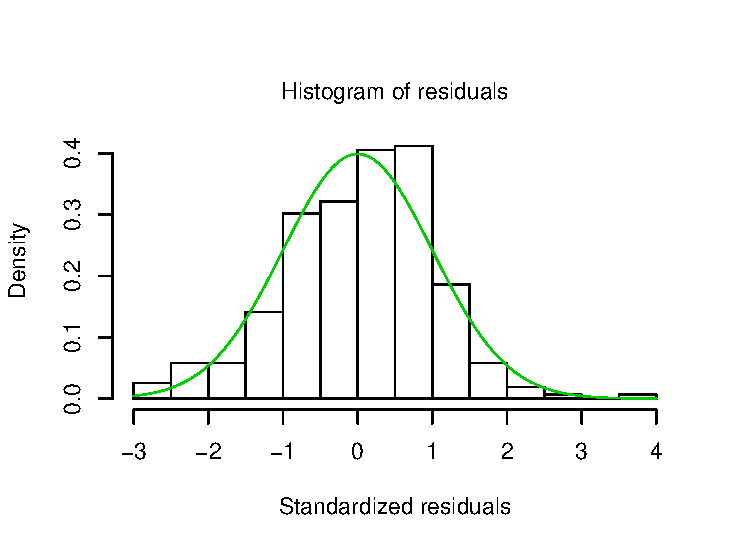
\includegraphics{img/img-unnamed-chunk-6-1} \end{center}

\end{CodeChunk}

\hypertarget{decomposition}{%
\subsection{Decomposition}\label{decomposition}}

As aforementioned the decomposition method differs between TRAMO-SEATS
and X-13ARIMA, where SEATS is based on ARIMA-model and X-11-algorithm on
linear filters. Consequently the composition of this object differs
between the two methods (tables \ref{tab:obj_tab_x13} and
\ref{tab:obj_tab_tramoseats}). The only common part is the first two
sub-objects with the model specification (\code{specification}) and
information on the decomposition mode (\code{mode}; e.g.: additive).

Then, the \code{decomposition_X11} object comprises quality measures on
the decomposition (\code{mstats}), namely the \(M\) and \(Q\)
statistics. It contains also the final unmodified S-I ratios \(d8\) and
final seasonal factors \(d10\) (\code{si_ratio}), as well as the
information on the final seasonal filter (\code{s_filter}) and trend
filter(\code{t_filter}). The code below presents the output for X-11
decomposition:

\begin{CodeChunk}

\begin{CodeInput}
R> sax13$decomposition
\end{CodeInput}

\begin{CodeOutput}
 Monitoring and Quality Assessment Statistics:  
      M stats
M(1)    0.028
M(2)    0.033
M(3)    0.338
M(4)    0.376
M(5)    0.366
M(6)    0.067
M(7)    0.066
M(8)    0.157
M(9)    0.073
M(10)   0.145
M(11)   0.120
Q       0.156
Q-M2    0.171

Final filters: 
Seasonal filter:  3x5
Trend filter:  13 terms Henderson moving average
\end{CodeOutput}
\end{CodeChunk}

As a reminder, in SEATS it is assumed that each component of the
linearized series (received from TRAMO) is an outcome of a linear
stochastic process and SEATS estimates an ARIMA model for each component
(i.e.~trend, seasonal, transitory and irregular). Therfore the
\code{decomposition_SEATS} object contains the information on the
estimated ARIMA models (\code{model}), the linearized components - as
obtained from TRAMO (\code{linearized}) - and the theoretical components
calculated from the ARIMA models (\code{components}). The code below
presents the output for the SEATS decomposition, with the information on
the ARIMA models:

\begin{CodeChunk}

\begin{CodeInput}
R> sats$decomposition
\end{CodeInput}

\begin{CodeOutput}
Model
AR :  1 + 0.094056 B - 0.158875 B^2 - 0.294600 B^3 
D :  1 - B - B^12 + B^13 
MA :  1 - 0.510600 B^12 


SA
AR :  1 + 0.094056 B - 0.158875 B^2 - 0.294600 B^3 
D :  1 - 2.000000 B + B^2 
MA :  1 - 0.937923 B - 0.015753 B^2 - 0.007005 B^3 + 0.015440 B^4 - 0.001104 B^5 
Innovation variance:  0.5777661 

Trend
AR :  1 - 0.711394 B 
D :  1 - 2.000000 B + B^2 
MA :  1 - 0.312018 B - 0.965498 B^2 + 0.346519 B^3 
Innovation variance:  0.07090723 

Seasonal
D :  1 + B + B^2 + B^3 + B^4 + B^5 + B^6 + B^7 + B^8 + B^9 + B^10 + B^11 
MA :  1 + 1.314878 B + 1.722951 B^2 + 2.227262 B^3 + 2.229462 B^4 + 2.119339 B^5 + 1.926456 B^6 + 1.615753 B^7 + 1.268615 B^8 + 0.770474 B^9 + 0.278823 B^10 - 0.025652 B^11 
Innovation variance:  0.08441922 

Transitory
AR :  1 + 0.805449 B + 0.414116 B^2 
MA :  1 - 0.452913 B - 0.547087 B^2 
Innovation variance:  0.02525112 

Irregular
Innovation variance:  0.07006354 
\end{CodeOutput}
\end{CodeChunk}

\hypertarget{final}{%
\subsection{Final}\label{final}}

The final object has a simple structure as it includes the input series,
final seasonally adjusted series and the final components (i.e.~\(t\) -
trend-cycle, \(s\) - seasonal component and \(i\) - irregular component)
(\code{series}), as well as their forecasts (\code{forecasts}).

\begin{CodeChunk}

\begin{CodeInput}
R> sats$final
\end{CodeInput}

\begin{CodeOutput}
Last observed values
             y       sa        t             s           i
Jan 2017  96.5 102.9317 102.6366  -6.431739755  0.29515069
Feb 2017  99.3 102.3815 102.7523  -3.081452963 -0.37082579
Mar 2017 110.5 103.2230 103.0587   7.276971010  0.16431902
Apr 2017 103.4 103.3950 103.4579   0.004977088 -0.06292068
May 2017 104.6 104.1023 103.8400   0.497657700  0.26230153
Jun 2017 107.7 103.8403 104.2863   3.859652578 -0.44596785
Jul 2017 107.6 105.1862 104.9032   2.413785110  0.28301107
Aug 2017  88.7 105.5484 105.5999 -16.848375561 -0.05151353
Sep 2017 112.1 106.2889 106.3305   5.811052841 -0.04159101
Oct 2017 113.4 106.9003 107.1101   6.499696169 -0.20982123
Nov 2017 114.3 108.3110 107.7487   5.988950554  0.56232415
Dec 2017 101.7 107.7534 108.1104  -6.053350690 -0.35709913

Forecasts:
               y_f     sa_f      t_f         s_f           i_f
Jan 2018 102.49061 108.4010 108.4016  -5.9103802 -0.0005820963
Feb 2018 105.85284 108.8666 108.7446  -3.0137577  0.1219532717
Mar 2018 116.21918 108.9840 109.0820   7.2351710 -0.0979861094
Apr 2018 108.90762 109.4437 109.4153  -0.5360850  0.0284199810
May 2018 110.11320 109.7634 109.7457   0.3498301  0.0176868066
Jun 2018 114.47710 110.0480 110.0740   4.4290998 -0.0260150048
Jul 2018 112.47723 110.4145 110.4009   2.0627149  0.0136293681
Aug 2018  93.98244 110.7265 110.7267 -16.7440681 -0.0002045225
Sep 2018 116.57469 111.0463 111.0518   5.5283721 -0.0054794124
Oct 2018 118.30580 111.3809 111.3764   6.9249450  0.0044980848
Nov 2018 117.56621 111.6992 111.7005   5.8670241 -0.0013538638
Dec 2018 105.59658 112.0237 112.0245  -6.4271099 -0.0007722619
\end{CodeOutput}
\end{CodeChunk}

\hypertarget{diagnostics}{%
\subsection{Diagnostics}\label{diagnostics}}

This part of the \code{sa_object} includes several diagnostics on the
presence of seasonality in the input series and on the quality of the
seasonal adjustment.

The tests for the seasonality presence (\code{combined_test}) are
performed both on the entire series and in the last 3 years.

As regards the seasonal adjustment quality checks, they are grouped into
two sets. The first looks at the contribution of each estimated
component to the variance of the original series
(\code{variance_decomposition}). The second verifies, with different
tests, that there is no seasonal pattern left in the seasonally adjusted
series and in the irregular component (\code{residuals_test}).

All the above checks (except \code{combined_seasonality_test}), together
with a detailed description, are displayed when printing the diagnostics
object.

\begin{CodeChunk}

\begin{CodeInput}
R> sats$diagnostics
\end{CodeInput}

\begin{CodeOutput}
 Relative contribution of the components to the stationary
 portion of the variance in the original series,
 after the removal of the long term trend 
 Trend computed by Hodrick-Prescott filter (cycle length = 8.0 years)
           Component
 Cycle        15.148
 Seasonal     83.993
 Irregular     0.174
 TD & Hol.     0.076
 Others        0.049
 Total        99.441

 Combined test in the entire series 
 Non parametric tests for stable seasonality
                                                          P.value
   Kruskall-Wallis test                                      0.000
   Test for the presence of seasonality assuming stability   0.000
   Evolutive seasonality test                                0.027
 
 Identifiable seasonality present

 Residual seasonality tests 
                                      P.value
 qs test on sa                          1.000
 qs test on i                           1.000
 f-test on sa (seasonal dummies)        1.000
 f-test on i (seasonal dummies)         1.000
 Residual seasonality (entire series)   1.000
 Residual seasonality (last 3 years)    0.999
 f-test on sa (td)                      0.994
 f-test on i (td)                       0.922
\end{CodeOutput}
\end{CodeChunk}

\hypertarget{user-def}{%
\subsection{User-defined}\label{user-def}}

As presented in the tables \ref{tab:obj_tab_x13} and
\ref{tab:obj_tab_tramoseats} and in the previous sections the
\code{sa_object} has a defined structure with a defined content.
Nevertheless users can also extract additional output from the seasonal
adjustment estimation and this will be stored under \code{user_defined}
object in a form of a list. In order to receive the additional output
extra variables need to be defined as characters under the argument
\code{userdefined} of the functions \code{x13()} or \code{tramoseats()}.

For example, to receive additionally tables \(c10\) and \(d16\) the
following need to be specified in the function argument:

\begin{CodeChunk}

\begin{CodeInput}
R> sa_usrdef <- x13(myseries, spec = "RSA3", 
R+                  userdefined = c("decomposition.c10", "decomposition.d16"))
R> sa_usrdef$user_defined
\end{CodeInput}

\begin{CodeOutput}
Names of additional variables (2):
decomposition.c10, decomposition.d16
\end{CodeOutput}
\end{CodeChunk}

The list of all available variables can be obtained with the following
functions:

\begin{itemize}
\item
  \code{user_defined_variables("X13-ARIMA")}
\item
  \code{user_defined_variables("TRAMO-SEATS")}
\end{itemize}

\hypertarget{user-def-spec}{%
\section{Model specification: creation and
modification}\label{user-def-spec}}

Users can also create their own specifications by modifying pre-defined
specifications (as described in tables \ref{tab:pre_def_ts} and
\ref{tab:pre_def_x13}) or previously defined specifications or models.
For that, there are two functions for each method (X-13ARIMA and
TRAMO-SEATS) - one for the RegARIMA model and one for the entire
seasonal adjustment:

\begin{itemize}
\tightlist
\item
  RegARIMA model: \code{regarima_spec_x13()} for X-13ARIMA and
  \code{regarima_spec_tramoseats()} for TRAMO-SEATS;
\item
  seasonal adjustment: \code{x13_spec()} for X-13ARIMA and
  \code{tramoseats_spec()} for TRAMO-SEATS.
\end{itemize}

As mentionned above, the input of the functions can be a pre-defined
\proglang{JDemetra+} model specification, previously modified
specification or a model.

Once the specification is created, the estimations can be performed for:

\begin{itemize}
\tightlist
\item
  RegARIMA model by \code{regarima()} and;
\item
  seasonal adjustment with X-13ARIMA by \code{x13()} and with
  TRAMO-SEATS by \code{tramoseats()}.
\end{itemize}

The example below ilustrates how to create its own RegARIMA model for
the TRAMO-SEATS method by adding an additive outlier in October 2009:

\begin{CodeChunk}

\begin{CodeInput}
R> regarima_ts_spec <- regarima_spec_tramoseats(spec = "TRfull",
R+              usrdef.outliersEnabled = TRUE,
R+              usrdef.outliersType = "AO",
R+              usrdef.outliersDate = "2009-10-01")
R> regarima_ts_model <- regarima(series = ipi_c_eu[, "EA19"],
R+                               spec = regarima_ts_spec)
R> regarima_ts_model
\end{CodeInput}

\begin{CodeOutput}
y = regression model + arima (3, 1, 0, 0, 1, 1)
Log-transformation: no
Coefficients:
          Estimate Std. Error
Phi(1)     0.09633      0.055
Phi(2)    -0.16551      0.055
Phi(3)    -0.29422      0.056
BTheta(1) -0.50637      0.051

             Estimate Std. Error
Monday       -0.23323      0.094
Tuesday      -0.01617      0.094
Wednesday     0.29430      0.095
Thursday     -0.35287      0.095
Friday        0.13248      0.094
Saturday      0.30763      0.095
AO (10-2009) -0.80480      0.787
AO (1-2016)   3.25565      0.807


Residual standard error: 1.226 on 311 degrees of freedom
Log likelihood = -506.6, aic =  1039 aicc =  1040, bic(corrected for length) = 0.6292
\end{CodeOutput}
\end{CodeChunk}

And how to modify the specification of the X-13ARIMA object
\code{sa_usrdef} (defined in section \ref{user-def}) by changing the
seasonal filter and performing a working day adjustment:

\begin{CodeChunk}

\begin{CodeInput}
R> sa_x13_spec <- x13_spec(spec = sa_usrdef,
R+                          tradingdays.option = "WorkingDays",
R+                          x11.seasonalma = "S3X3")
R> sa_x13_model <- x13(series = ipi_c_eu[, "EA19"],
R+                     spec = sa_x13_spec)
\end{CodeInput}
\end{CodeChunk}

Almost all the specification variables available in \proglang{JDemetra+}
can be used in \pkg{RJDemetra}. For more details see the help page for
the corresponding function or the documentation of \proglang{JDemetra+}.

To prevent from wrong user specification, there are automatic checks in
\pkg{RJDemetra}, like in \proglang{JDemetra+}. For example, to
pre-specify an outlier or a user-defined variable you have to enable
them (setting the parameter \code{usrdef.outliersEnabled} or
\code{usrdef.varEnabled} to \code{TRUE}); or to fix the coefficient of
an outlier or a user-defined regressor you have to specify the
transformation function (\code{transform.function}, it cannot be
automatic). Those checks are done each time a new specification is
created. Therefore, some specifications cannot be set in two stages. For
example, fixing the coefficient of an outlier has to be done at the same
time when the outliers are defined. The following code doesn't fix the
coefficient of the outlier previously defined for January 2001:

\begin{CodeChunk}

\begin{CodeInput}
R> regarima_wrong_spec <- regarima_spec_tramoseats(spec = regarima_ts_model,
R+              transform.function = "Log",
R+              usrdef.outliersCoef =  -0.8)
\end{CodeInput}
\end{CodeChunk}

To fix it you have to re-define the outlier:

\begin{CodeChunk}

\begin{CodeInput}
R> regarima_good_spec <- regarima_spec_tramoseats(spec = regarima_ts_model,
R+              transform.function = "Log",
R+              usrdef.outliersType = "AO",
R+              usrdef.outliersDate = "2009-10-01",
R+              usrdef.outliersCoef =  -0.8)
\end{CodeInput}
\end{CodeChunk}

The documentation for the functions used to modify specifications
provide information on the interdependencies between different
arguments. The package offers also functions to display different parts
of the model specification. These are presented under the entry
\code{specification} of the package documentation. For instance, from
the example above, we can check which user defined variables were
enabled and with which parameters.

In the first case (wrongly specified), an outlier was pre-defined but
its coefficient was not fixed:

\begin{CodeChunk}

\begin{CodeInput}
R> s_usrdef(regarima_wrong_spec)
\end{CodeInput}

\begin{CodeOutput}
 outlier outlier.coef variables variables.coef
    TRUE        FALSE     FALSE          FALSE
\end{CodeOutput}

\begin{CodeInput}
R> s_preOut(regarima_wrong_spec)
\end{CodeInput}

\begin{CodeOutput}
  type       date coeff
1   AO 2009-10-01    NA
\end{CodeOutput}
\end{CodeChunk}

In the second case, the coefficient was correctly fixed:

\begin{CodeChunk}

\begin{CodeInput}
R> s_usrdef(regarima_good_spec)
\end{CodeInput}

\begin{CodeOutput}
 outlier outlier.coef variables variables.coef
    TRUE         TRUE     FALSE          FALSE
\end{CodeOutput}

\begin{CodeInput}
R> s_preOut(regarima_good_spec)
\end{CodeInput}

\begin{CodeOutput}
  type       date coeff
1   AO 2009-10-01  -0.8
\end{CodeOutput}
\end{CodeChunk}

\hypertarget{manipulate-workspace}{%
\section[Manipulate JDemetra+ workspaces]{Manipulate \proglang{JDemetra+} workspaces}\label{manipulate-workspace}}

\pkg{RJDemetra} allows to interact with \proglang{JDemetra+} workspaces
that can be opened by the software. A workspace includes:

\begin{itemize}
\tightlist
\item
  An XML file that enables users to import a workspace to
  \proglang{JDemetra+} and to display its content;\\
\item
  A folder containing several sub-folders that correspond to different
  types of items created by the user.
\end{itemize}

Each workspace can contain several multi-processings and each
multi-processing stores results of the seasonal adjustment procedure
performed with the TRAMO-SEATS or X-13ARIMA methods.

Exporting models to workspace allows to store easily the seasonal
adjustment models, to change specifications with the
\proglang{JDemetra+} graphical interface and to give models to users
unfamiliar with \proglang{R}.

\hypertarget{export-wk}{%
\subsection{Export a workspace}\label{export-wk}}

Four functions can to be used to export models:

\begin{itemize}
\tightlist
\item
  \code{new_workspace()} to create a workspace;\\
\item
  \code{new_multiprocessing()} to create a multi-processing in a
  workspace;\\
\item
  \code{add_sa_item()} to add a seasonal adjustment model to a
  multi-processing;\\
\item
  \code{save_workspace()} to export the workspace.
\end{itemize}

The following commands export seasonal adjustment models computed by
TRAMO-SEATS and X-13ARIMA:

\begin{CodeChunk}

\begin{CodeInput}
R> myseries <- ipi_c_eu[, "EA19"]
R> sa_x13 <- x13(myseries)
R> sa_ts <- tramoseats(myseries)
\end{CodeInput}
\end{CodeChunk}

First, to create a workspace and a multi-processing named ``MP-1'' the
following need to be executed:

\begin{CodeChunk}

\begin{CodeInput}
R> wk <- new_workspace()
R> new_multiprocessing(wk, name = "MP-1")
\end{CodeInput}
\end{CodeChunk}

Then, the two models will be added in the multiprocessing ``MP1'': the
name of the seasonal adjustment model computed with X-13ARIMA will be
``SA with X13'' and the one with TRAMO-SEATS will be ``SA with
TramoSeats'':

\begin{CodeChunk}

\begin{CodeInput}
R> add_sa_item(wk, multiprocessing = "MP-1",
R+             sa_obj = sa_x13, name =  "SA with X13")
R> add_sa_item(wk, multiprocessing =  "MP-1",
R+             sa_obj = sa_ts, name = "SA with TramoSeats")
\end{CodeInput}
\end{CodeChunk}

The exported workspace is named ``workspace.xml'':

\begin{CodeChunk}

\begin{CodeInput}
R> dir <- tempdir()
R> save_workspace(wk, file =  file.path(dir, "workspace.xml"))
\end{CodeInput}
\end{CodeChunk}

\hypertarget{import-a-workspace}{%
\subsection{Import a workspace}\label{import-a-workspace}}

The following functions can be used to import a workspace:

\begin{itemize}
\tightlist
\item
  \code{load_workspace()} to load a workspace;\\
\item
  \code{compute()} to compute multi-processings: by default a workspace
  contains only definitions, therfore computation is needed to get the
  seasonal adjustment model;\\
\item
  \code{get_model()} to get the seasonal adjustment models;\\
\item
  \code{get_ts()} to get the input raw time series, \code{get_object()}
  and \code{get_all_objects} to navigate inside a workspace (extract a
  multi-processing or a seasonal adjustment model), \code{get_name()} to
  get names of the multiprocessings or the seasonal adjustment models,
  and \code{count()} to count the number of multiprocessings or seasonal
  adjustment models.
\end{itemize}

For instance, the following need to be run to import the workspace
created in section \ref{export-wk} and to get the first multiprocessing
and the first seasonal adjustment model:

\begin{CodeChunk}

\begin{CodeInput}
R> wk <- load_workspace(file =  file.path(dir, "workspace.xml"))
R> mp1 <- get_object(wk, 1)
R> sa_item1 <- get_object(mp1, 1)
\end{CodeInput}
\end{CodeChunk}

To get the number of seasonal adjustment models in the multiprocessing:

\begin{CodeChunk}

\begin{CodeInput}
R> count(mp1)
\end{CodeInput}

\begin{CodeOutput}
[1] 2
\end{CodeOutput}
\end{CodeChunk}

And to receive the name of the first seasonal adjustment model in
\proglang{JDemetra+}:

\begin{CodeChunk}

\begin{CodeInput}
R> get_name(sa_item1) 
\end{CodeInput}

\begin{CodeOutput}
[1] "SA with X13"
\end{CodeOutput}
\end{CodeChunk}

Finally, raw time series and seasonal adjustment model can now be
imported:

\begin{CodeChunk}

\begin{CodeInput}
R> raw_ts <- get_ts(sa_item1)
R> compute(wk)
R> sa_model1 <- get_model(sa_item1, workspace = wk)
\end{CodeInput}
\end{CodeChunk}

\code{get_ts()} and \code{get_model()} can also be used directly on a
workspace or on a multiprocessing to import all the raw time series or
all the seasonal adjustment model:

\begin{itemize}
\tightlist
\item
  for a multiprocessing the result is a list which each element contains
  the information on the seasonal adjustment model;\\
\item
  for a workspace the result is a list of number of multi-processings
  length and which each element contains a list with the information on
  each seasonal adjustment model.
\end{itemize}

For example to get all raw time series of the workspace and all seasonal
adjustment models of the first multi-processing the following need to be
run:

\begin{CodeChunk}

\begin{CodeInput}
R> all_raw_ts <- get_ts(wk)
R> sa_models_of_mp1 <- get_model(mp1, workspace = wk)
\end{CodeInput}
\end{CodeChunk}

The imports of seasonal adjustment models from a workspace work well
when they have been created through \pkg{RJDemetra}. Troubles might
occur when importing a workspace created with \proglang{JDemetra+}, in
particular:

\begin{itemize}
\tightlist
\item
  Seasonal adjustment models with ramp effect or intervention variables
  will be partially imported: the result of the imported model will be
  correct but changing the specification (through \code{x13_spec()} or
  \code{tramoseats_spec()}) will erase them.\\
\item
  Seasonal adjustment models with no pre-processing (X-11 specification)
  are not supported: \code{NULL} object will be returned.
\end{itemize}

\hypertarget{advanced-usage-and-examples}{%
\section{Advanced usage and
examples}\label{advanced-usage-and-examples}}

By default, \code{x13()}, \code{tramoseats()} and \code{regarima()}
export a large number of diagnostics and indicators. This might be
time-consuming, especially when dealing with many series and only a few
indicators are needed. To customise the output and receive only the
needed indicators, four functions extracting the associated seasonal
adjustment Java model can be used: \code{jx13()}, \code{jtramoseats()},
\code{jregarima_x13()} and \code{jregarima_tramoseats()}. Three other
functions can be used to manipulate these objects:

\begin{itemize}
\tightlist
\item
  \code{get_dictionary()} to get the list of indicators that can be
  extracted;\\
\item
  \code{get_indicators()} to get selected indicators;\\
\item
  \code{jSA2R()} to get the corresponding formatted seasonal adjustment
  or RegARIMA model.
\end{itemize}

For example to only receive the seasonally adjusted time series:

\begin{CodeChunk}

\begin{CodeInput}
R> sa_jx13 <- jx13(myseries)
R> head(get_dictionary(sa_jx13))
\end{CodeInput}

\begin{CodeOutput}
[1] "y"    "y_f"  "t"    "t_f"  "sa"   "sa_f"
\end{CodeOutput}

\begin{CodeInput}
R> sa_series <- get_indicators(sa_jx13, "sa")
R> plot(sa_series[["sa"]])
\end{CodeInput}


\begin{center}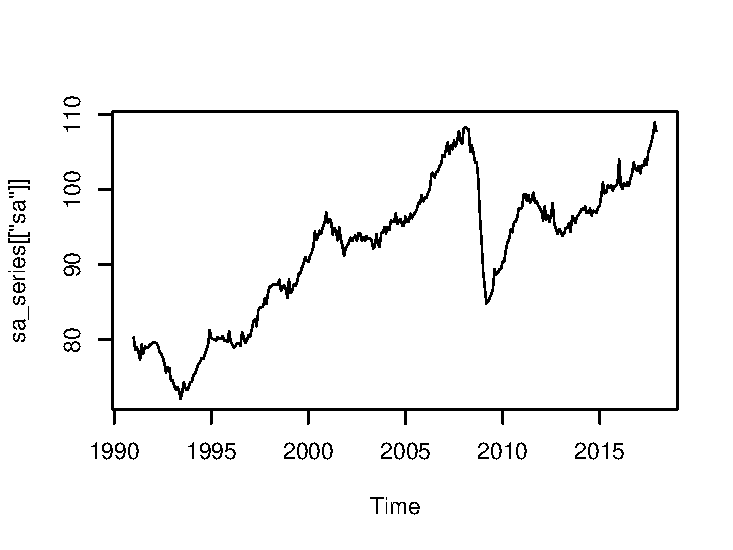
\includegraphics{img/img-unnamed-chunk-27-1} \end{center}

\end{CodeChunk}

To compute the revisions of the seasonal adjusted series of January 2010
with an automatic modelling:

\begin{CodeChunk}

\begin{CodeInput}
R> dates <- window(time(myseries), start = 2010)
R> revisions_history_j10 <- sapply(dates,function(last_date){
R+   sa_jx13 <- jx13(window(myseries, end = last_date))
R+   window(get_indicators(sa_jx13, "sa")[["sa"]],
R+          start = 2010,
R+          end = 2010)
R+ })
R> revisions_history_j10 <- ts(revisions_history_j10,
R+                             start = 2010, frequency = 12)
R> plot(revisions_history_j10)
\end{CodeInput}


\begin{center}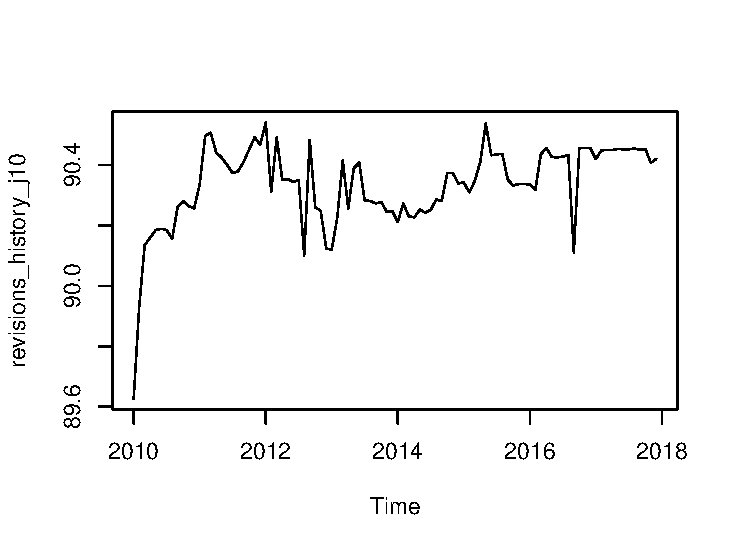
\includegraphics{img/img-unnamed-chunk-28-1} \end{center}

\end{CodeChunk}

When performing seasonal adjustment on a large database, the most common
error results from the preliminary check (used to verify the quality of
the input series) when excluding highly problematic series (with too
many identical observations and/or missing values). In this case, the
\code{jx13()} function will not give an error but
\code{get_indicators()} will only return a \code{NULL} objects:

\begin{CodeChunk}

\begin{CodeInput}
R> identical_ts <- ts(0,start = 2010, end = 2015, frequency = 12)
R> get_indicators(jx13(identical_ts), "sa", "sa_f")
\end{CodeInput}

\begin{CodeOutput}
$sa
NULL

$sa_f
NULL
\end{CodeOutput}
\end{CodeChunk}

To disable this preliminary check, you need to create a new
specification with the parameter \texttt{preliminary.check\ =\ FALSE}:

\begin{CodeChunk}

\begin{CodeInput}
R> myspec <- x13_spec(preliminary.check = FALSE)
R> my_indicators <- get_indicators(jx13(identical_ts, myspec)
R+                                 , "sa", "sa_f")
\end{CodeInput}
\end{CodeChunk}

This might be useful when performing large scale seasonal adjustment.
For example with our database on industrial production indices:

\begin{CodeChunk}

\begin{CodeInput}
R> ipi_sa_series <- lapply(colnames(ipi_c_eu),function(series){
R+   sa_jx13 <- jx13(ipi_c_eu[,series], myspec)
R+   get_indicators(sa_jx13, "sa")[["sa"]]
R+ })
R> ipi_sa_series <- do.call(ts.union,ipi_sa_series)
R> colnames(ipi_sa_series) <- colnames(ipi_c_eu)
\end{CodeInput}
\end{CodeChunk}

\hypertarget{conclusion}{%
\section{Conclusion}\label{conclusion}}

\proglang{JDemetra+} is a powerful tool for seasonal and trading days
adjustments. It implements the two leading methods, TRAMO-SEATS and
X-13ARIMA, through a rich graphical interface. Besides seasonal
adjustment, JDemetra+ bundles other time series models that are useful
in the production or analysis of economic statistics, including for
instance outlier detection, nowcasting, temporal disaggregation or
benchmarking. It is also the only software officially recommended by
Eurostat for seasonal and calendar adjustment.

Therefore, the package \pkg{RJDemetra}, being based on the same
libraries of JDemetra+, uses certified and tested algorithms. It also
offers huge opportunities to producers and researchers. Indeed,
\proglang{JDemetra+} being widely used in production, it allows to:

\begin{itemize}
\tightlist
\item
  Easily create tools that can be used in production. For example
  \pkg{rjdqa} \citep{rjdqa} reproduces Statistics Canada dashboard, used
  to provide a snapshot snapshot of an single seasonal adjustment model
  at a point in time and to point out some possible problems.\\
\item
  Customize the outputs to the need of the producers of a specific
  institution. For example to goal of \pkg{persephone}
  \citep{persephone} is to have enable easy processing during production
  of seasonally adjusted series in Statistics Austria.\\
\item
  Extend the current \proglang{R} package to use the same seasonal
  adjustment methods used in production. For example \pkg{ggdemetra}
  \citep{ggdemetra} extend the \pkg{ggplot2} \citep{ggplot2} to add
  seasonal adjustment statistics to plots (diagnostics, outliers, ARIMA
  models, seasonally adjusted series, etc.).
\end{itemize}

Moreover, directly manipulate the Java objects makes \pkg{RJDemetra}
much more performant than others \proglang{R} packages, specially with
large scale seasonal adjustment or to conduct studies.

The package \pkg{RJDemetra} will also evolved with \proglang{JDemetra+}
and integrate the new developments on seasonal adjustment methods, for
example the future extension of the methods to series of all frequencies
(weekly, daily, etc.).

\renewcommand\refname{References}
\bibliography{biblio.bib}


\end{document}

